\chapter{Organización}

\section{Introducción}

\section{Nombre}
Unidad Para la Atención y Reparación Integral a las Víctimas
\subsection{Misión}
Liderar acciones del Estado y la sociedad para atender y reparar integralmente a las víctimas, para contribuir a la inclusión social y a la paz.
\subsection{Visión}
En el 2021, habremos logrado que las víctimas, reparadas integralmente, ejerzan su ciudadanía y aporten en la consolidación de la paz como resultado de la gestión efectiva y coordinada de la Unidad con los demás actores del Sistema.
\newpage
\subsection{Proceso de negocio}
Gestión de la Información
\subsection{Objetivos}
\textbf{Objetivo Proceso}
\\Gestionar los servicios, gobierno y capacidad tecnológica que soporta la operación y las necesidades de la Unidad frente las tecnologías de la información y articular a las entidades que conforman la red nacional de información para facilitar el flujo eficiente de información que permita realizar el seguimiento a la implementación de la política pública a través de la gestión técnica, administrativa y financiera del personal del proceso frente a los dominios de: estrategia TI, gestión TI, servicios tecnológicos, sistemas de información, información, uso y apropiación y seguridad de la información frente a todos los procesos, y la gestión con las entidades externas y procesos misionales y estratégicos de la Unidad facilitando el flujo eficiente de la información con el fin de apoyar el cumplimiento de la misión y objetivos de la Unidad.
\\

\textbf{Objetivo Procedimiento}
\\Establecer la secuencia de actividades requeridas para desarrollar nuevos sistemas de información y/o funcionalidades en los existentes según los requerimientos de la Unidad para la Atención y Reparación Integral a las Víctimas, atendiendo las mejores
prácticas sugeridas por las guías técnicas que para el dominio de sistemas de información son publicadas por el Ministerio de Tecnologías de la Información - MINTIC.
\newpage
\subsection{Organigrama}
\begin{figure}[h!]
	\centering
	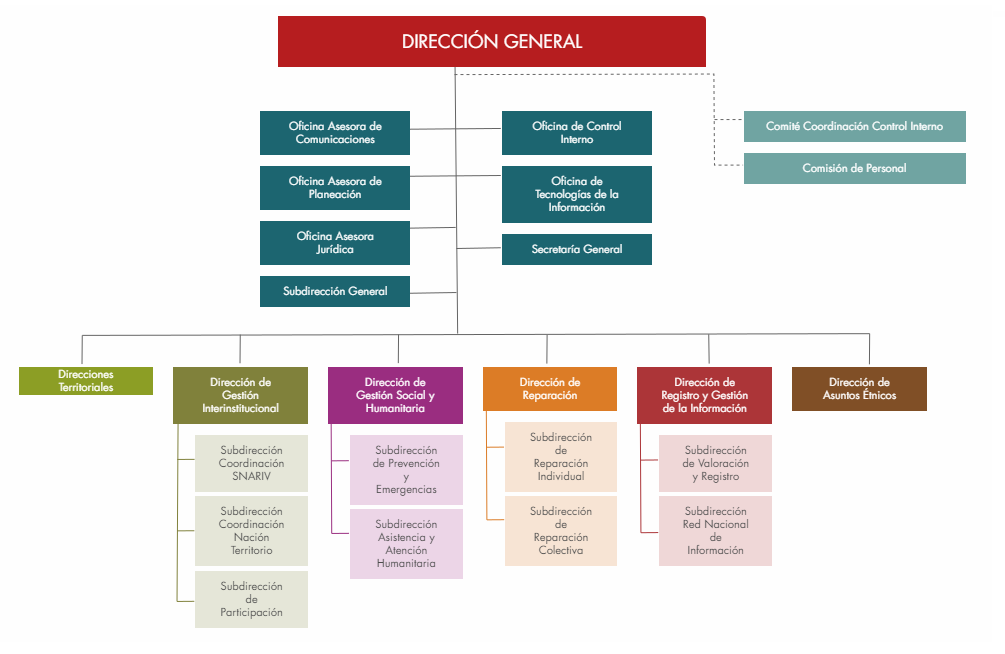
\includegraphics[width=0.7\linewidth]{Proyecto/Organizacion/imgs/Organigrama}
	\caption{}
\end{figure}

\subsection{Roles/Responsabilidades}
\begin{description}

\item[$\bullet$] Jefe de la Oficina de Tecnologías de la Información – OTI o quien haga sus veces.
\item[$\bullet$]Líder de Gestión Presupuestal de la OTI.
\item[$\bullet$]Líder Enlace de Planeación de la OTI
\item[$\bullet$]Líder de Sistemas de Información
\item[$\bullet$]Líder de Servicios Tecnológicos de la OTI
\item[$\bullet$]Líder de Infraestructura de la OTI
\item[$\bullet$]Líder de Uso y Apropiación de la OTI
\item[$\bullet$]Líder de la Seguridad de la Información de la OTI
\item[$\bullet$]Delegado de la Oficina Asesora de Comunicaciones
\item[$\bullet$]Delegado de la Subdirección Red Nacional de Información
\item[$\bullet$]Delegado de la Subdirección de Valoración y Registro 
\end{description}

\subsection{Producto}
\textbf{Prototipo meta- modelo de minería de datos para auditoría caso de estudio: Unidad para la atención y reparación integral a las víctimas del conflicto armado en Colombia.}